\chapter{Data-driven results}\label{ch:data-driven-results}
In this section we present the results of the data-driven models.
We go through two main cases. 
The first case is the 1D shallow water equations with Gaussian initial conditions, where we compare the performance of the CNN and FNO models.
The second case is the 1D linearized shallow water equations in spherical coordinates, where we compare the performance of the CNN and FNO models.
We also compare the performance of the models for different values of $\sigma$, i.e., the standard deviation of the Gaussian function.
We do this to see how the models perform for different types of initial conditions, depending how smooth or discontinuous the solution is.

\section{1D SWE with Gaussian initial conditions}
We start by showing the numerical solution of the shallow water equations, then we present the predictions of the NN and FNO models.
Until now, we have mostly considered discountinuous initial conditions, but we will also consider smooth initial conditions in this section.
We solve the SWE with the following initial conditions:
\begin{equation}\label{eq:data-driven-initial-conditions-gauss}
    \begin{aligned}
        h(x, 0) &= h_0 \exp \left( \frac{-{(x-\mu)}^2}{2 \sigma^2} \right) ,\\
        u(x, 0) &= 0 , \\
    \end{aligned}
\end{equation}
where $h_0 = 1, \mu = 0.5, \sigma = 0.1$. 
The function $h(x, 0)$ is a Gaussian function, illustrated in Figure~\ref{fig:NN_initial_1D}.
\begin{figure}[H]
    \centering
    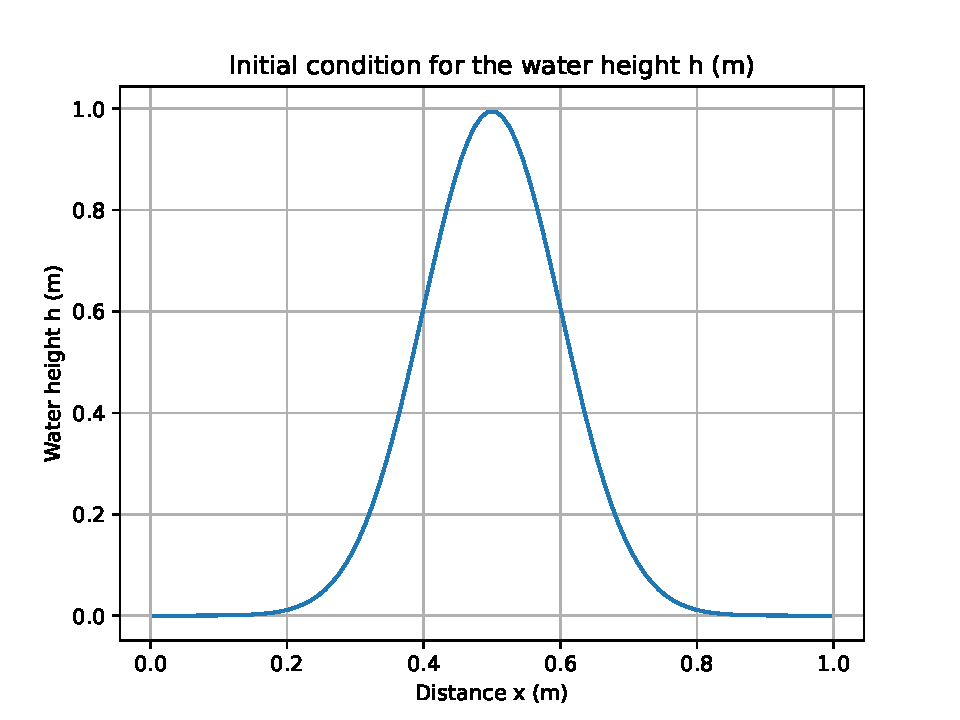
\includegraphics[width=0.5\textwidth]{C:/Users/Matteo/Shallow-Water-Equations/plots/NN_initial_1D.pdf}
    \caption{Initial conditions~\eqref{eq:data-driven-initial-conditions-gauss}.} \label{fig:NN_initial_1D}
\end{figure}
The domain is $ x \in [0, 1]$ with $N = 200$ points and the final time is $t = 1.0$.
We use a CFL number of $0.9$ and variable time steps.
The numerical solution is shown in Figure~\ref{fig:NN_initial}, in both a contour plot and a 3D plot.
\begin{figure}[H]
    \centering
    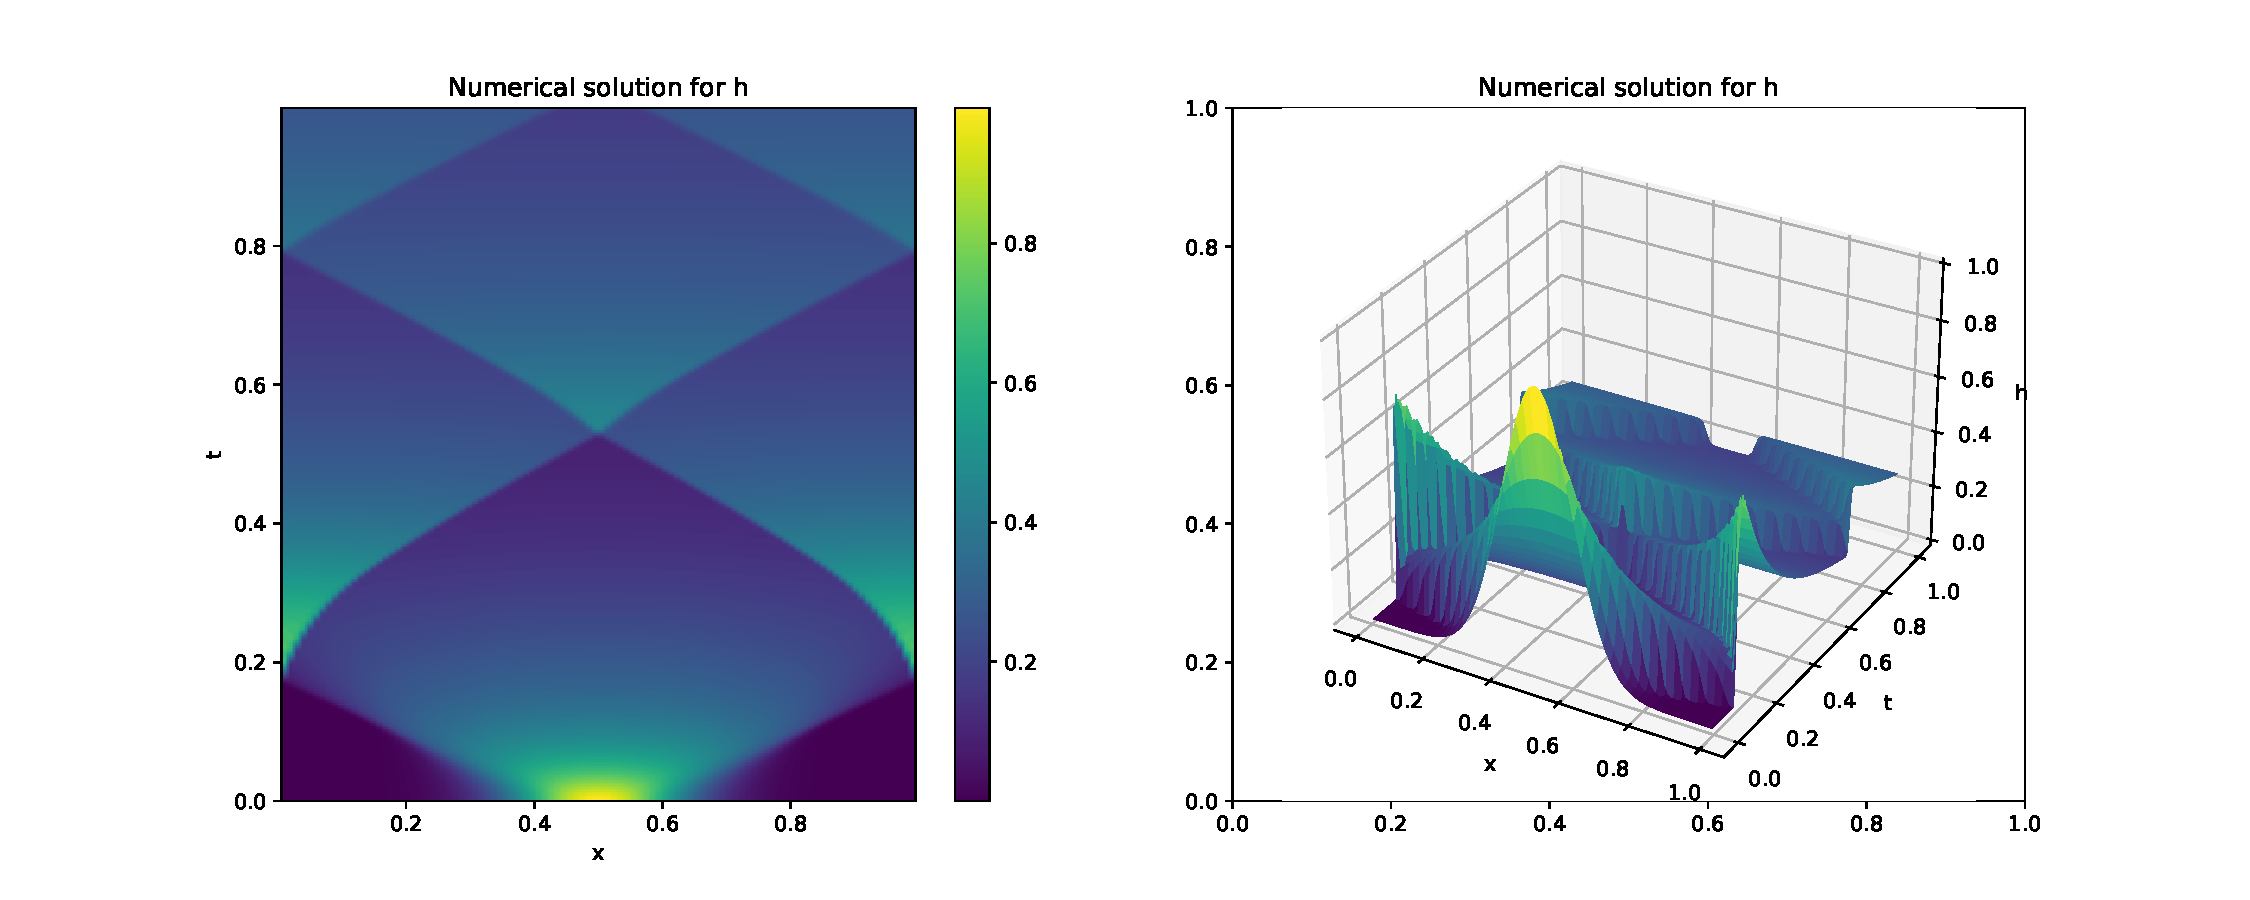
\includegraphics[width=0.7\textwidth]{C:/Users/Matteo/Shallow-Water-Equations/plots/NN_initial.pdf}
    \caption{Numerical solution of the shallow water equations with initial conditions~\eqref{eq:data-driven-initial-conditions-gauss}.}\label{fig:NN_initial}
\end{figure}


\subsection*{CNN Model}
%\addcontentsline{toc}{subsection}{Test case 1}
In the convolutional neural network, we train the model using the data generated by the numerical solution of the shallow water equations.
The model uses the data from the numerical solution to predict the solution at the next time step.
Meaning that the input and output data are the same, but shifted one time step.
This way, the model is supposed to learn the flowmap.
The model has been trained using the Adam optimizer with a learning rate of $0.001$, a batch size of $32$.

\begin{figure}[H]
    \centering
    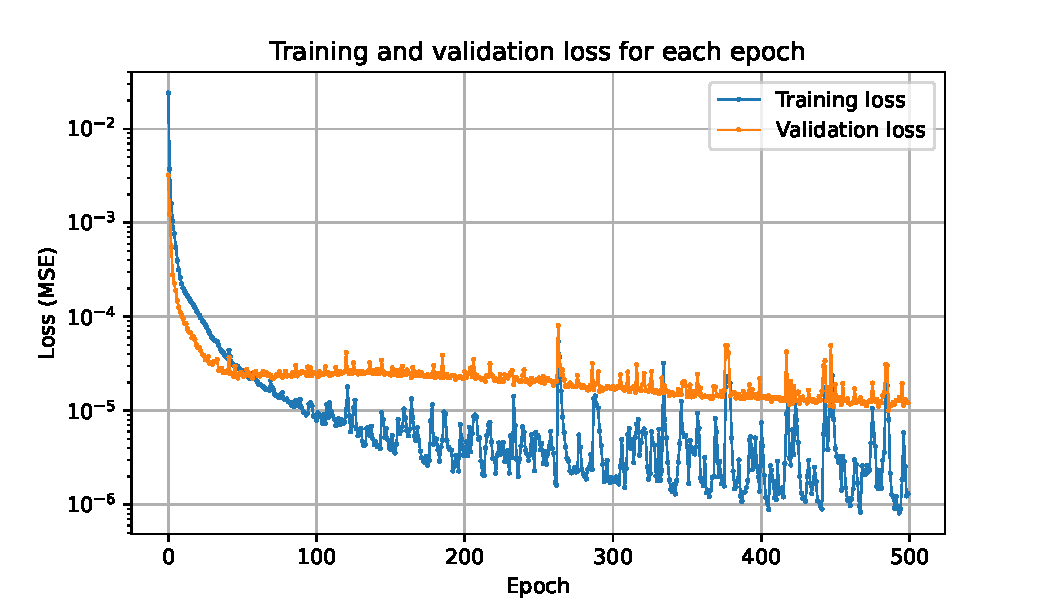
\includegraphics[width=0.7\textwidth]{C:/Users/Matteo/Shallow-Water-Equations/plots/1D_CNN_loss.pdf}
    \caption{Training and validation loss for the CNN model.}\label{fig:1D_CNN_loss}
\end{figure}


\begin{figure}[H]
    \centering
    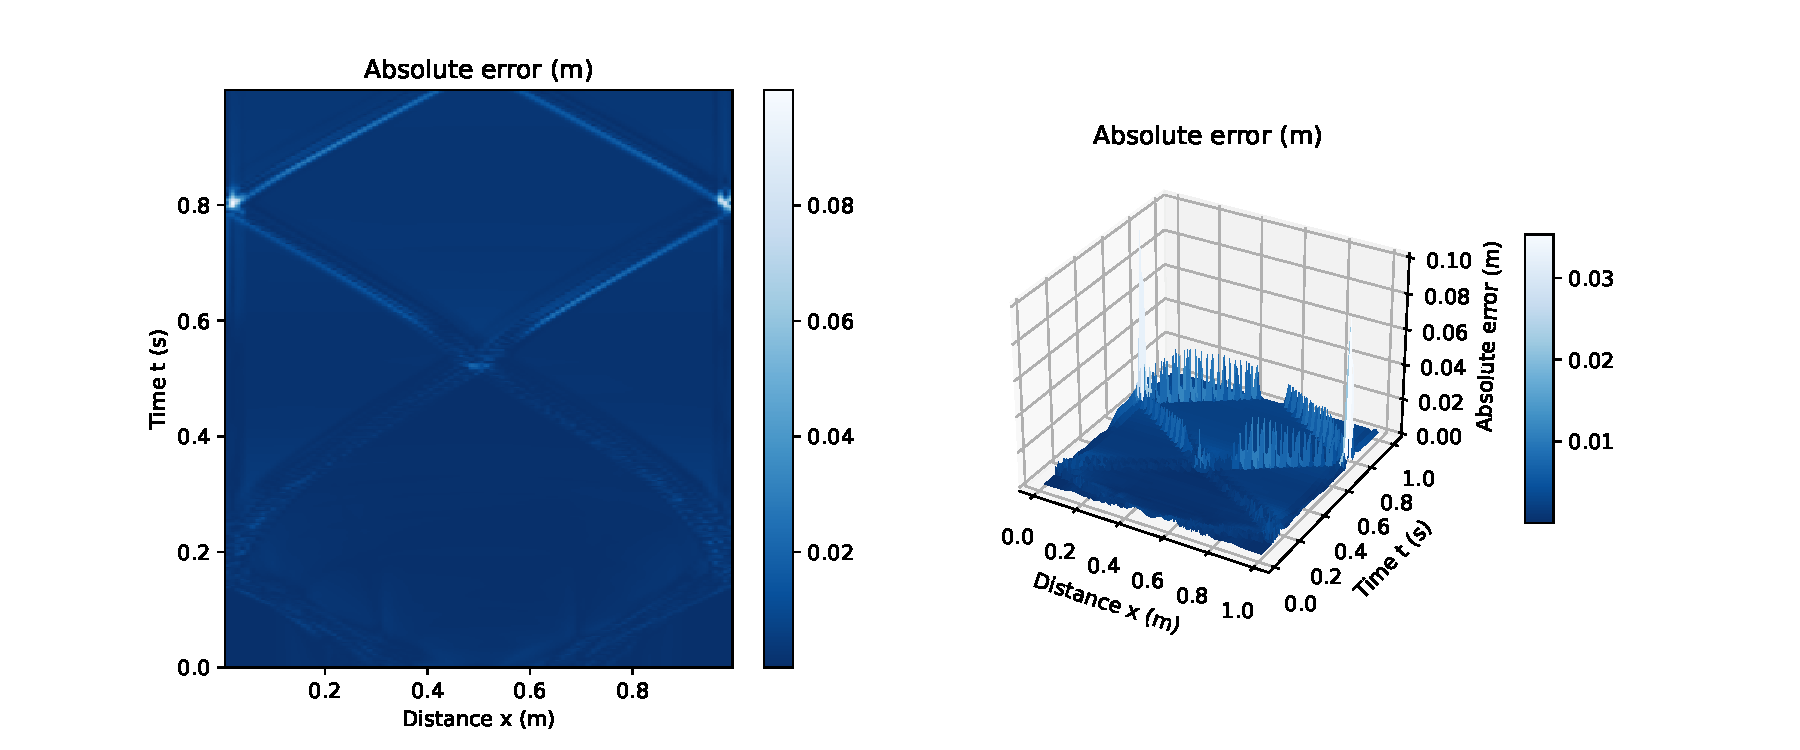
\includegraphics[width=\textwidth]{C:/Users/Matteo/Shallow-Water-Equations/plots/1D_CNN_error.pdf}
    \caption{Error plot for the predictions for the CNN model.}\label{fig:1D_CNN_error}
\end{figure}

To understand the performance of the model, we consider the predictions for some given time steps, shown in Figure~\ref{fig:1D_CNN_pred_timesteps}.

\begin{figure}[H]
    \centering
    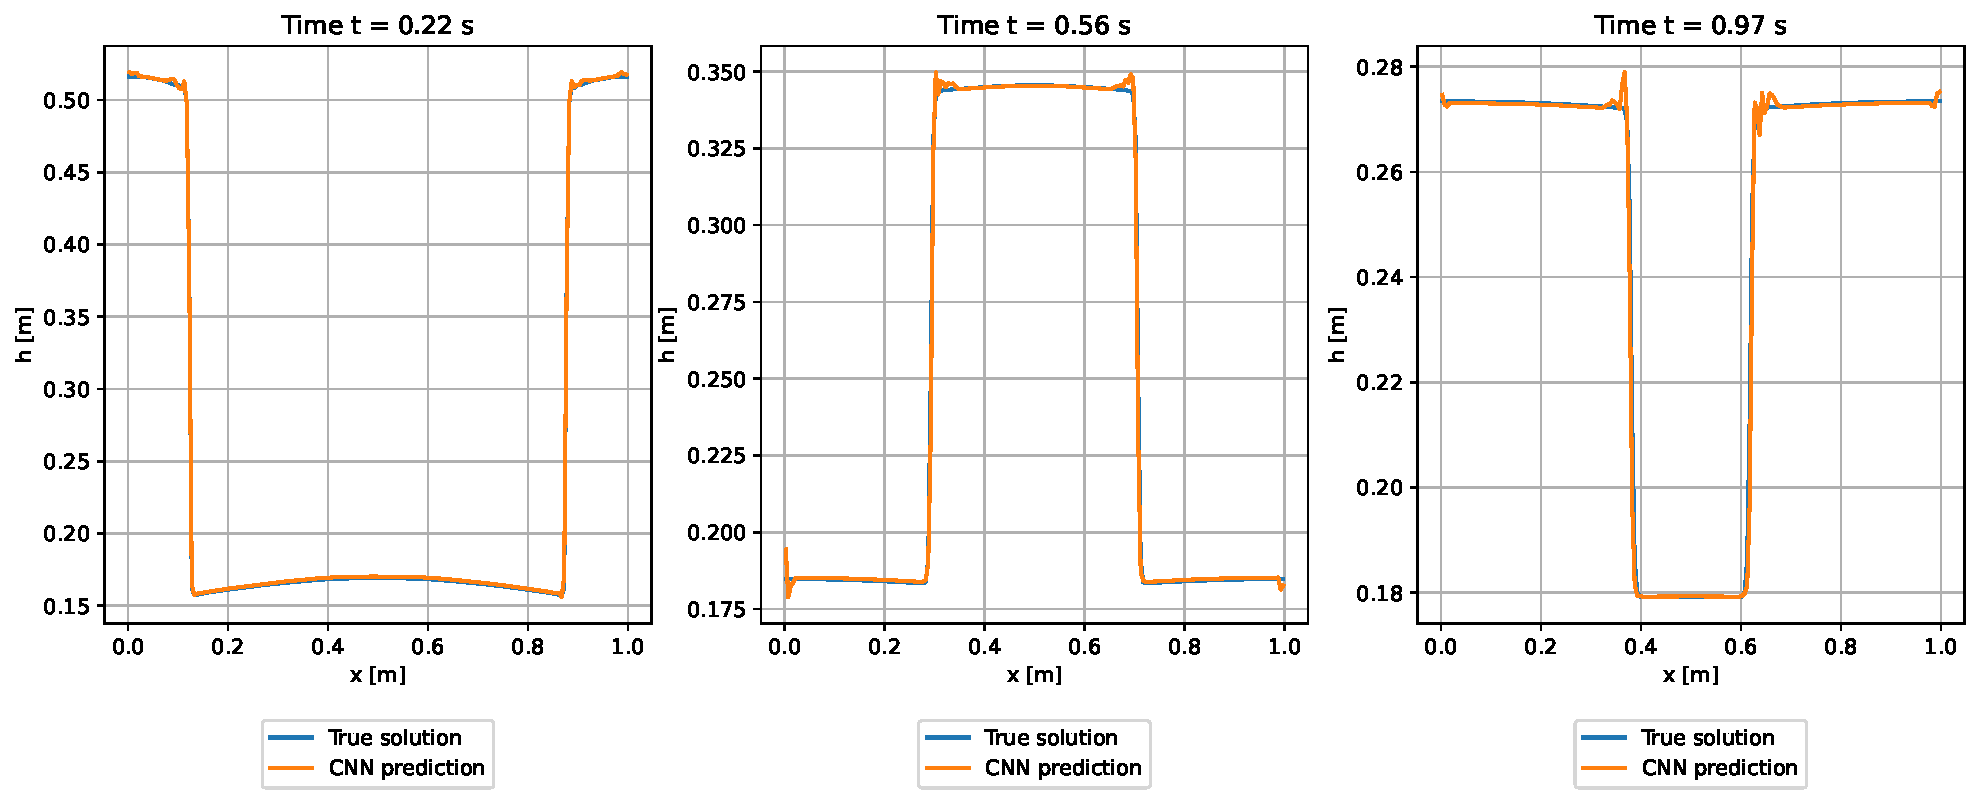
\includegraphics[width=\textwidth]{C:/Users/Matteo/Shallow-Water-Equations/plots/1D_CNN_pred_timesteps.pdf}
    \caption{Predictions for the CNN model for some given time steps.}\label{fig:1D_CNN_pred_timesteps}
\end{figure}

We also see that the highest absolute errors are located at the edges of the solution, which is expected, as the solution tends to be discontinuous.
We also see that the further we get in time, the worse the predictions become. This is also somehow expected, since we are outside the training data.

Based on the training and validation loss, the model is overfitting the data. We see that as the training loss is decreasing, the validation loss is increasing.
This also means that the model is not able to generalize the data.
A possible solution could be to use more data.

Again, we see that the model finds some of the dynamics, but has many oscillations.
We have also trained a FNN model and a LSTM model, but the results are not shown here, as the performance is worse than the RNN model.

\subsection*{FNO Model}
One of the main goals in this thesis is to use Fourier Neural Operators to solve the shallow water equations.
We define a FNO model, which consists of an input channel, 64 hidden channels and an output channel. We use a Fourier basis with 16 modes and a batch size of 32.
The model is trained using the Adam optimizer with a learning rate of $0.001$, a total of $1000$ epochs and the critera is to minimize the mean squared error (MSE).
The model is trained on the same data as the CNN model, and tested on the same data.

\begin{figure}[H]
    \centering
    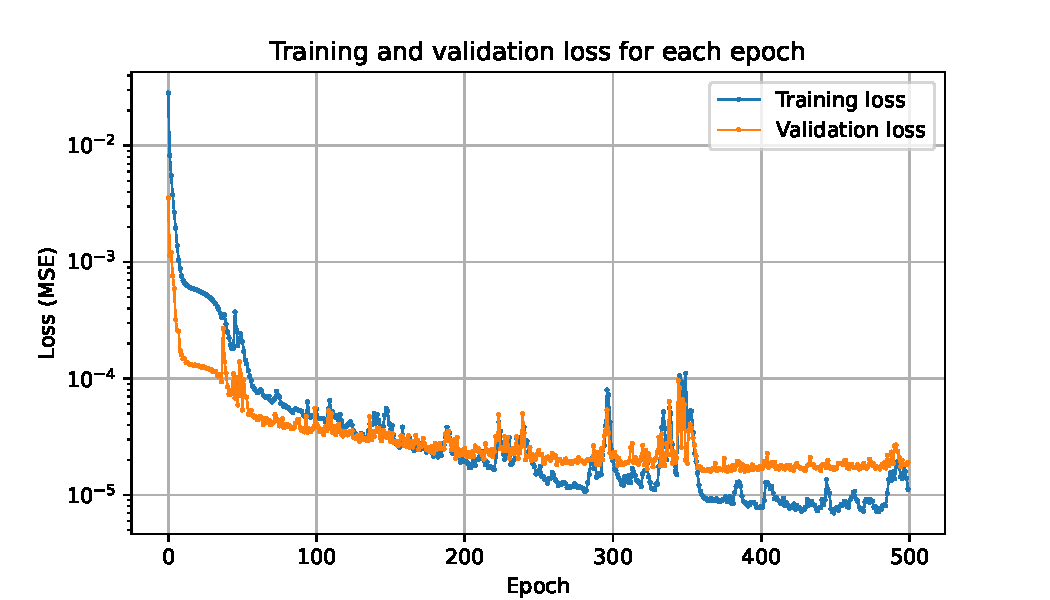
\includegraphics[width=0.7\textwidth]{C:/Users/Matteo/Shallow-Water-Equations/plots/1D_FNO_loss.pdf}
    \caption{Training and validation loss for the FNO model.}\label{fig:1D_FNO_loss}
\end{figure}

\begin{figure}[H]
    \centering
    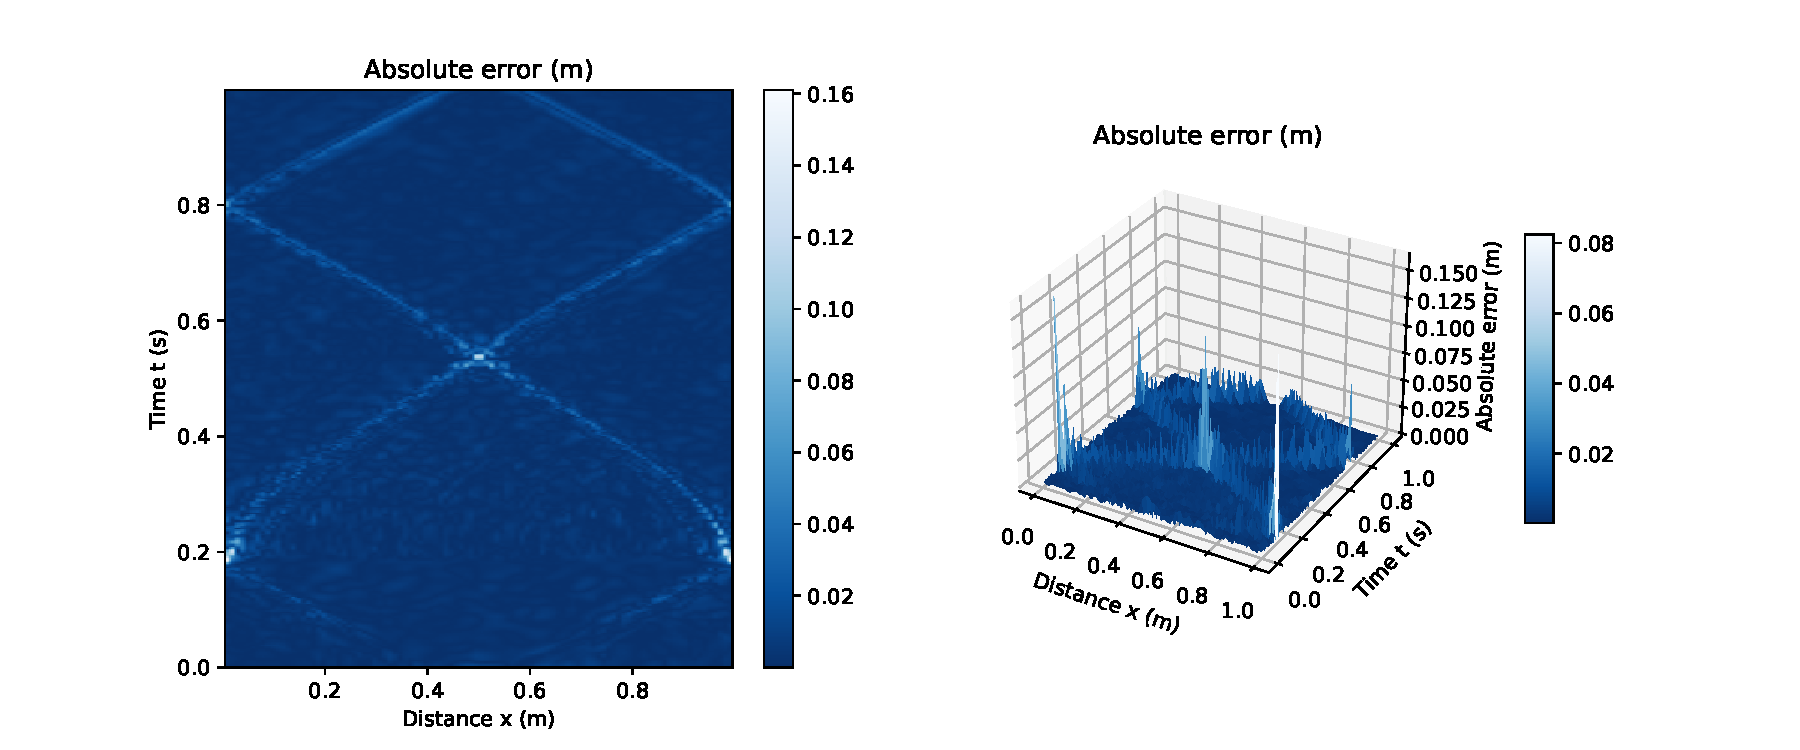
\includegraphics[width=\textwidth]{C:/Users/Matteo/Shallow-Water-Equations/plots/1D_FNO_error.pdf}
    \caption{Error plot for the predictions for the FNO model.}\label{fig:1D_FNO_error}
\end{figure}

To get an overview of the performance of the model, we consider the predictions for some given time steps, shown in Figure~\ref{fig:1D_FNO_pred_timesteps}.
\begin{figure}[H]
    \centering
    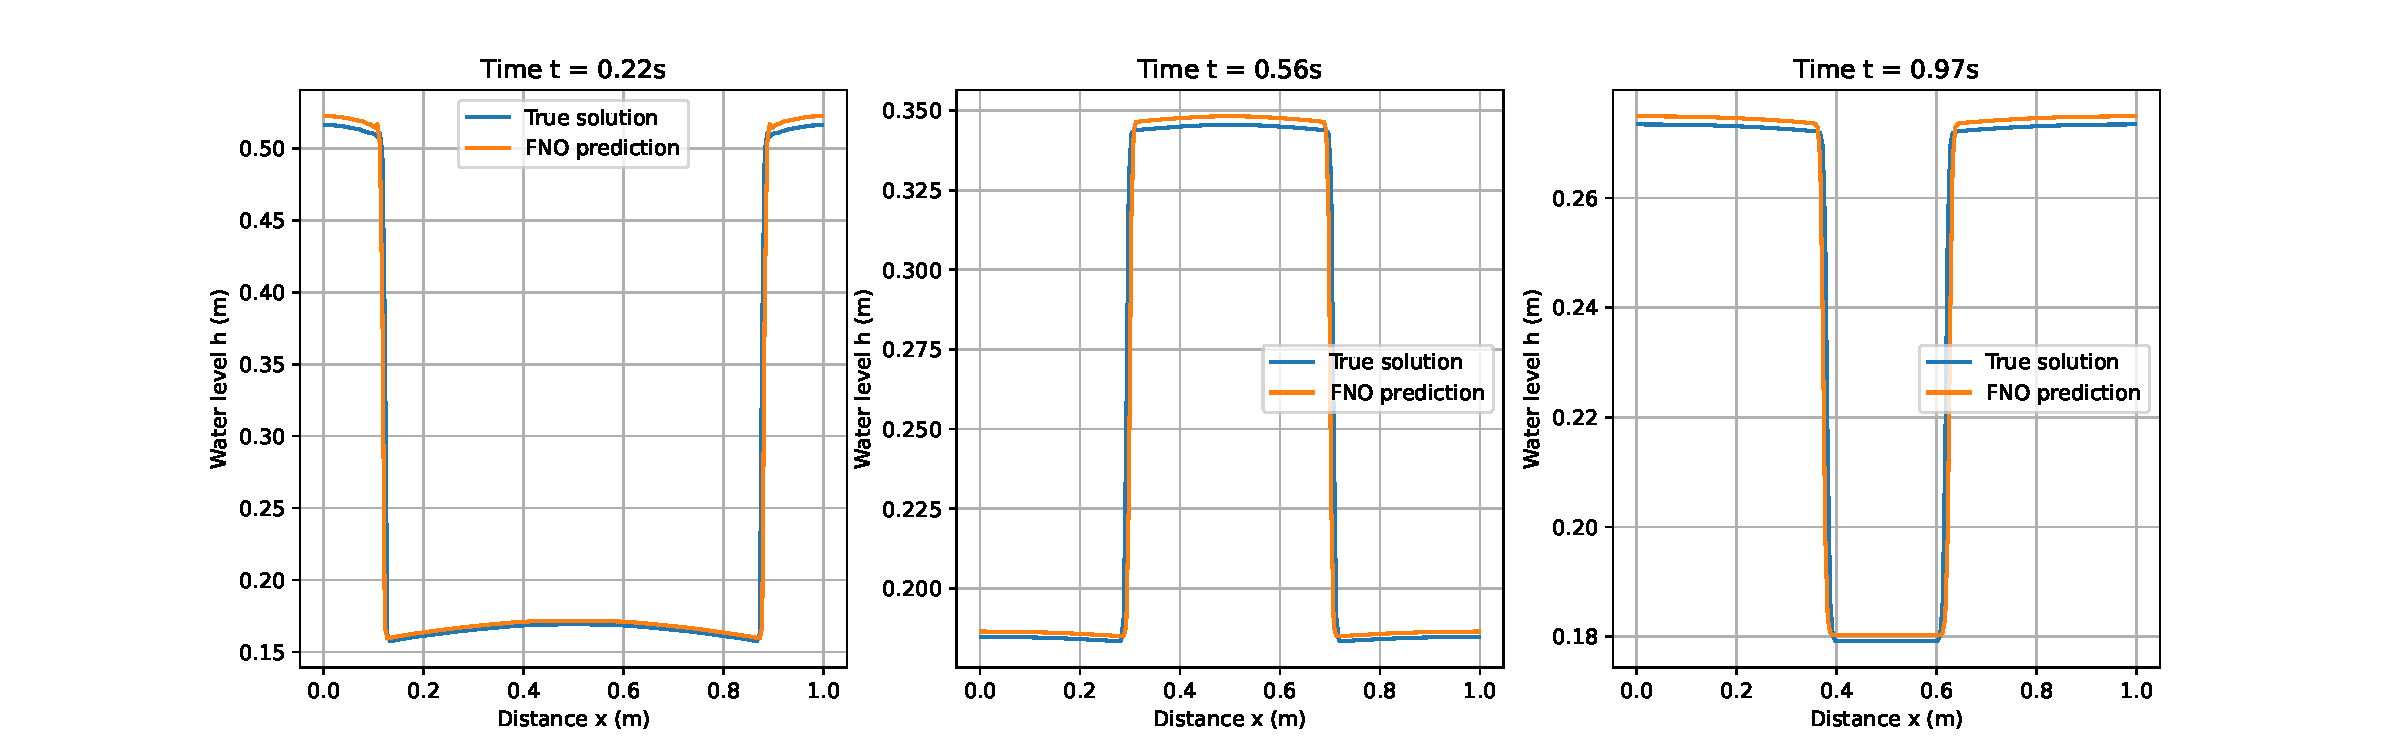
\includegraphics[width=\textwidth]{C:/Users/Matteo/Shallow-Water-Equations/plots/1D_FNO_pred_timesteps.pdf}
    \caption{Predictions for the FNO model for some given time steps.}\label{fig:1D_FNO_pred_timesteps}
\end{figure}


\subsection*{Comparison}
UDFYLDT MED 1D CNN Gauss + 1D FNO Gauss (ikke for Toro).
\begin{table}[H]
    \centering
    \small % Reduce font size
    \begin{tabular}{c|cccc|cccc}
        Model & \multicolumn{4}{c|}{Gauss initial condition} & \multicolumn{4}{c}{Toro test case} \\
        \cline{2-9}
        & Epochs & MSE & MAE & Time (s) & Epochs & MSE & MAE & Time (s) \\
        \hline
        CNN  &
        \input{C:/Users/Matteo/Shallow-Water-Equations/saved_results/1D_CNN_nepochs.txt} &
        \input{C:/Users/Matteo/Shallow-Water-Equations/saved_results/1D_CNN_MSE_test.txt} & 
        \input{C:/Users/Matteo/Shallow-Water-Equations/saved_results/1D_CNN_MAE_test.txt} &
        \input{C:/Users/Matteo/Shallow-Water-Equations/saved_results/1D_CNN_time.txt} &
        \input{C:/Users/Matteo/Shallow-Water-Equations/saved_results/2D_CNN_Nx=100_nepochs.txt} &
        \input{C:/Users/Matteo/Shallow-Water-Equations/saved_results/2D_CNN_Nx=100_MSE_test.txt} &
        \input{C:/Users/Matteo/Shallow-Water-Equations/saved_results/2D_CNN_Nx=100_MAE_test.txt} &
        \input{C:/Users/Matteo/Shallow-Water-Equations/saved_results/2D_CNN_Nx=100_time.txt} 
        \\
        \hline
        FNO  &
        \input{C:/Users/Matteo/Shallow-Water-Equations/saved_results/1D_FNO_nepochs.txt} &
        \input{C:/Users/Matteo/Shallow-Water-Equations/saved_results/1D_FNO_MSE_test.txt} &
        \input{C:/Users/Matteo/Shallow-Water-Equations/saved_results/1D_FNO_MAE_test.txt} &
        \input{C:/Users/Matteo/Shallow-Water-Equations/saved_results/1D_FNO_time.txt} &
        \input{C:/Users/Matteo/Shallow-Water-Equations/saved_results/2D_CNN_Nx=100_nepochs.txt} &
        \input{C:/Users/Matteo/Shallow-Water-Equations/saved_results/2D_FNO_Nx=100_MSE_test.txt} &
        \input{C:/Users/Matteo/Shallow-Water-Equations/saved_results/2D_FNO_Nx=100_MAE_test.txt} &
        \input{C:/Users/Matteo/Shallow-Water-Equations/saved_results/2D_FNO_Nx=100_time.txt}
        \\
        \hline
    \end{tabular}
    \caption{Test loss in terms of MSE and MAE, and time for training the models for the 2D SWE.}\label{tab:results_2D_comparison}
\end{table}




\section{1D linearized SWE in Spherical Coordinates}
We also consider the spherical shallow water equations in a 1D setting, focusing on the linearized SWE on a circular domain.
The length of the domain corresponds to the circumreference of the circle, $L = 2\pi$, and is discretized into $N = 500$ points.
The initial conditions is specified as a Gaussian function wrapped around the circle, expressed as:
\begin{align*}
    h(\theta, 0) &= h_0 \exp \left( \frac{-{(\theta-\mu)}^2}{2 \sigma^2} \right) ,\\
\end{align*}
where the parameters are $h_0 = 1, \mu = \frac{\pi}{4}, \sigma = \frac{\pi}{16}$.
The initial conditions can be seen in \autoref{fig:swe_spherical_1d_initial_conditions}.
\begin{figure}[H]
    \centering
    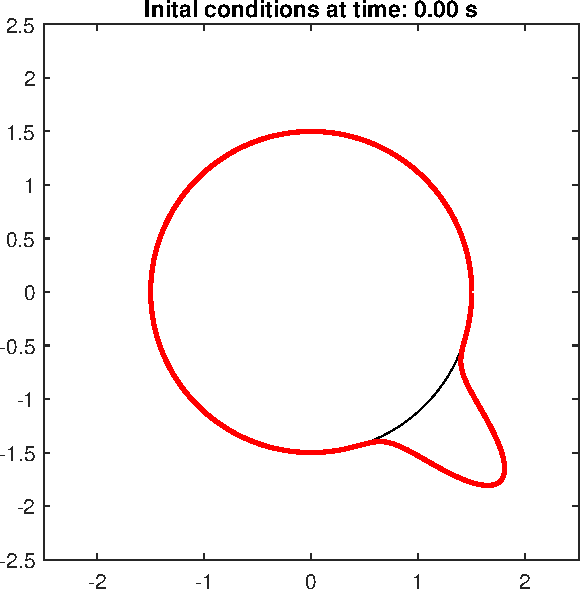
\includegraphics[width=0.4\textwidth]{C:/Users/Matteo/Shallow-Water-Equations/plots/SWE-spherical-1d-initial_conditions.pdf}
    \caption{Initial conditions for the 1D linearized shallow water equations in spherical coordinates.}\label{fig:swe_spherical_1d_initial_conditions}
\end{figure}
The numerical solution in the $\theta,t$ plane is shown in \autoref{fig:Spherical_linear_1D_true_solution}, for $t=0$ to $t=1$.
\begin{figure}[H]
    \centering
    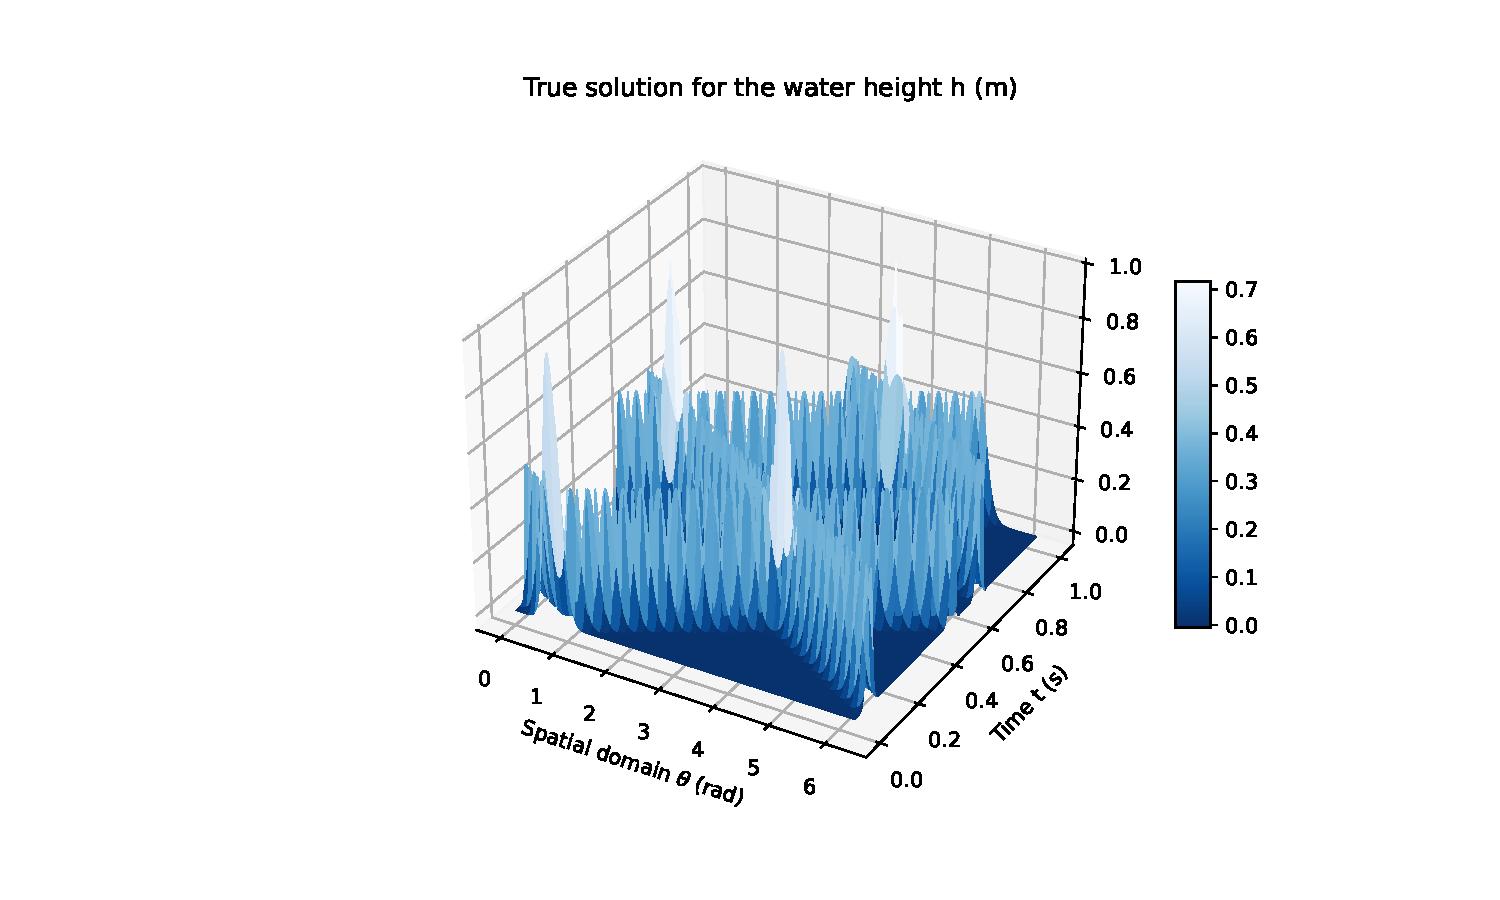
\includegraphics[width=0.8\textwidth]{C:/Users/Matteo/Shallow-Water-Equations/plots/Spherical_linear_1D_true_solution.pdf}
    \caption{Numerical solution of the spherical shallow water equations in 1D in the $\theta,t-$space.}\label{fig:Spherical_linear_1D_true_solution}
\end{figure}
Based on the data generated by the numerical solution (we use time steps of $\Delta t = 0.0025$), we train a FNO model and a Convolutional Neural Network (CNN) model.

\subsubsection*{CNN Model}
We have also trained a CNN model on the data generated by the numerical solution of the SWE in 1D.
Like the FNO model, the CNN model is trained on the data from $t = 0$ to $t = 0.6$, validated on the data from $t = 0.6$ to $t = 0.8$, and tested on the data from $t = 0.8$ to $t = 1.0$.
The training and validation loss is shown in \autoref{fig:1D_CNN_sphere_loss}.
\begin{figure}[H]
    \centering
    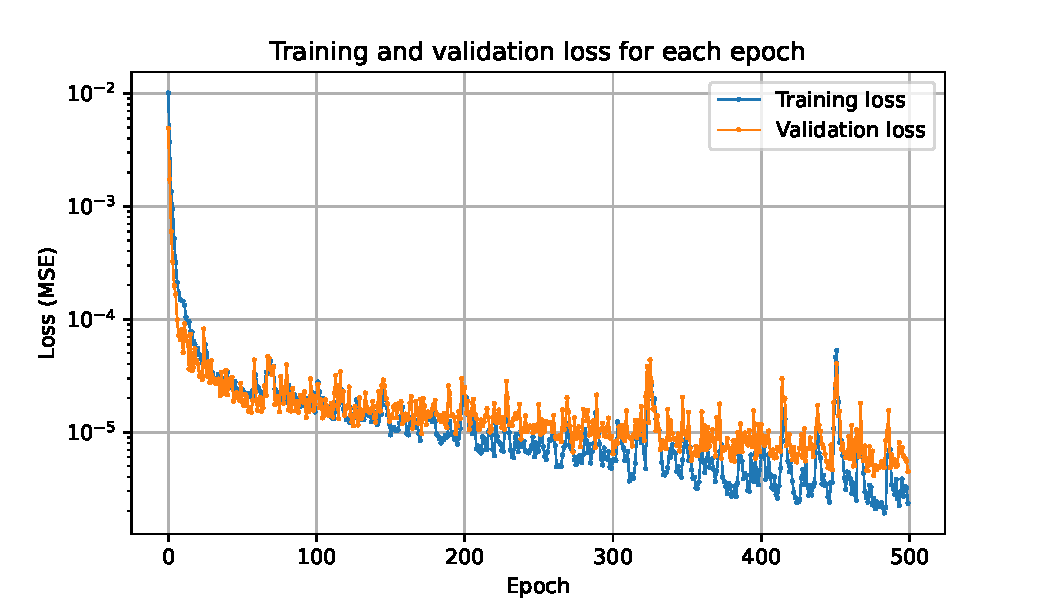
\includegraphics[width=0.7\textwidth]{C:/Users/Matteo/Shallow-Water-Equations/plots/1D_CNN_sphere_loss.pdf}
    \caption{Training and validation loss for the CNN model for the spherical shallow water equations in 1D.}\label{fig:1D_CNN_sphere_loss}
\end{figure}
The error plots are shown in \autoref{fig:1D_CNN_sphere_error}.
\begin{figure}[H]
    \centering
    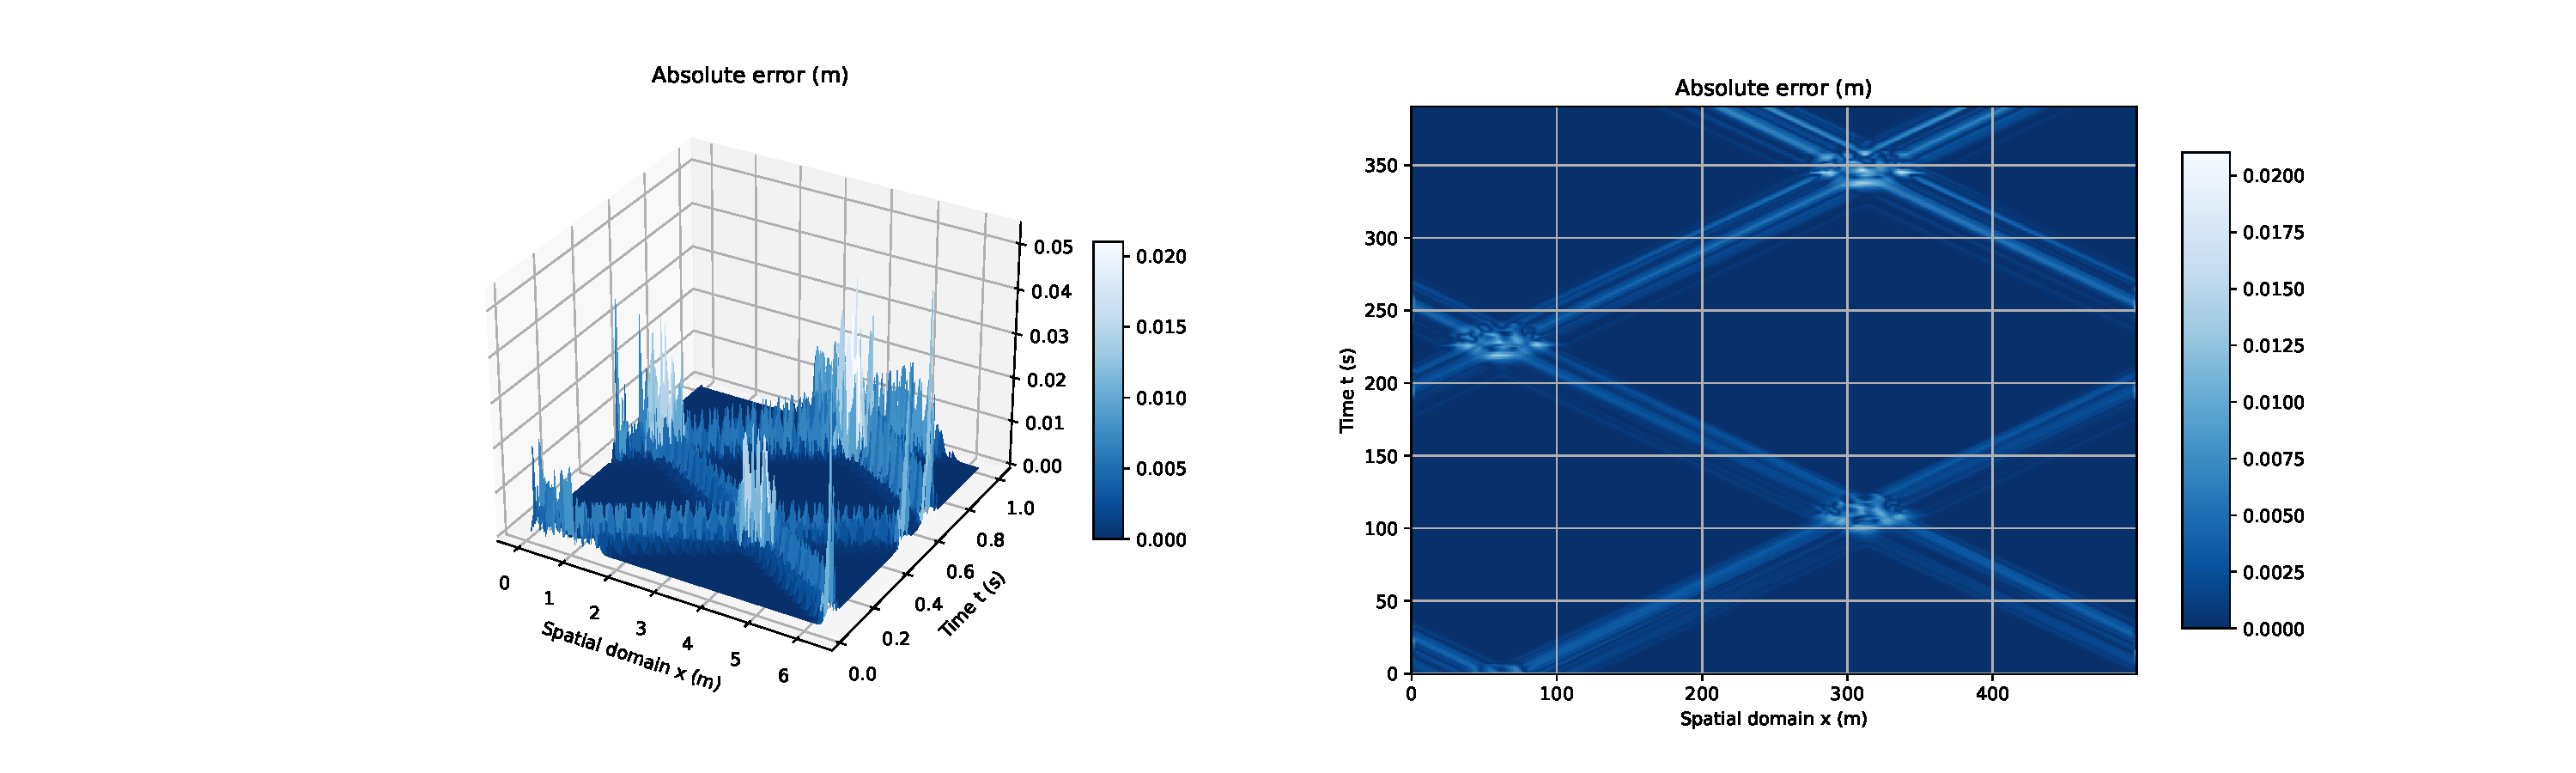
\includegraphics[width=\textwidth]{C:/Users/Matteo/Shallow-Water-Equations/plots/1D_CNN_sphere_error_sigma=2.pdf}
    \caption{Error plots for the predictions of the CNN model for solving the 1D linearized spherical SWE.}\label{fig:1D_CNN_sphere_error}
\end{figure}
The predictions for some given time steps are shown in \autoref{fig:1D_CNN_sphere_pred_timesteps_sigma=2}.
\begin{figure}[H]
    \centering
    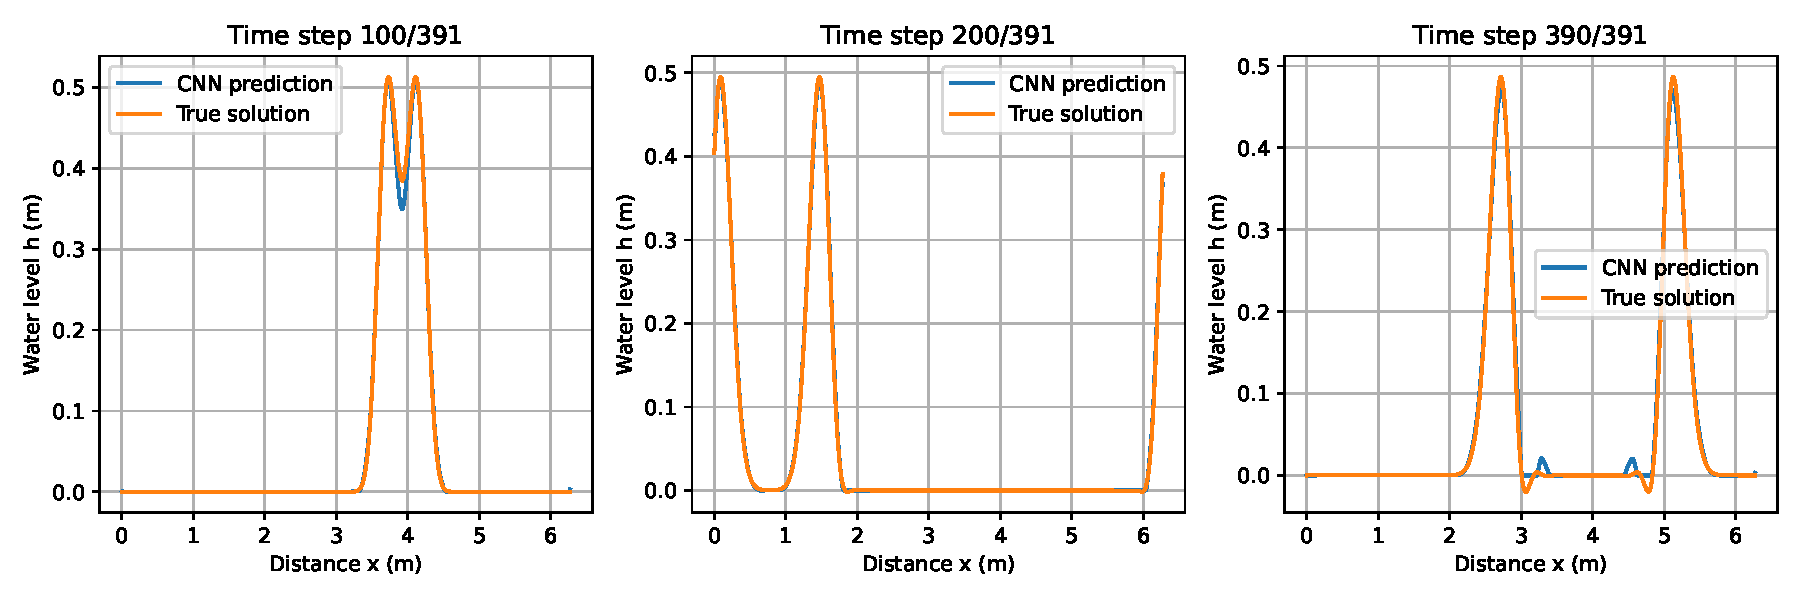
\includegraphics[width=0.9\textwidth]{C:/Users/Matteo/Shallow-Water-Equations/plots/1D_CNN_sphere_pred_timesteps_sigma=2.pdf}
    \caption{Predictions for the spherical shallow water equations in 1D using the CNN model for some given time steps.}\label{fig:1D_CNN_sphere_pred_timesteps_sigma=2}
\end{figure}
From \autoref{fig:1D_CNN_sphere_pred_timesteps_sigma=2}, we also see that the predictions capture the waves, but are more noisy than the FNO predictions.

\subsubsection*{FNO model}
The FNO model consists of an input channel, 64 hidden channels and an output channel. We use a Fourier basis with 16 modes and a batch size of 32.
The model is trained using the Adam optimizer with a learning rate of $0.001$, a total of $100$ epochs and the critera is to minimize the mean squared error (MSE).
The model is trained on the data from $t = 0$ to $t = 0.6$, validated on the data from $t = 0.6$ to $t = 0.8$, and tested on the data from $t = 0.8$ to $t = 1.0$.
The training and validation loss is shown in \autoref{fig:1D_FNO_sphere_loss}.
\begin{figure}[H]
    \centering
    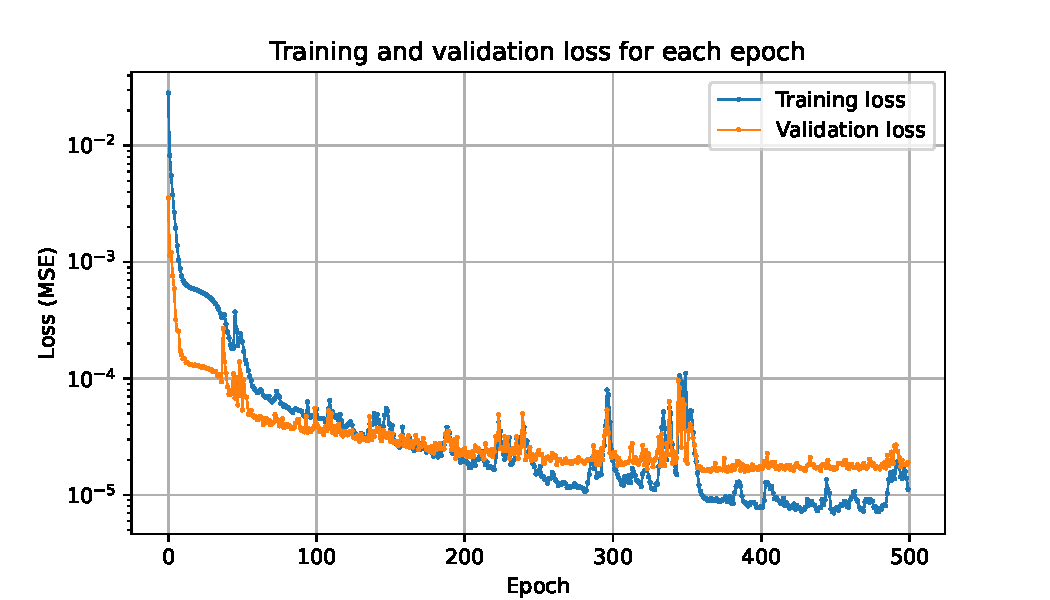
\includegraphics[width=0.7\textwidth]{C:/Users/Matteo/Shallow-Water-Equations/plots/1D_FNO_loss.pdf}
    \caption{Training and validation loss for the FNO model for the spherical shallow water equations in 1D.}\label{fig:1D_FNO_sphere_loss}
\end{figure}
The error plots are shown in \autoref{fig:1D_FNO_sphere_error_sigma=2}.
\begin{figure}[H]
    \centering
    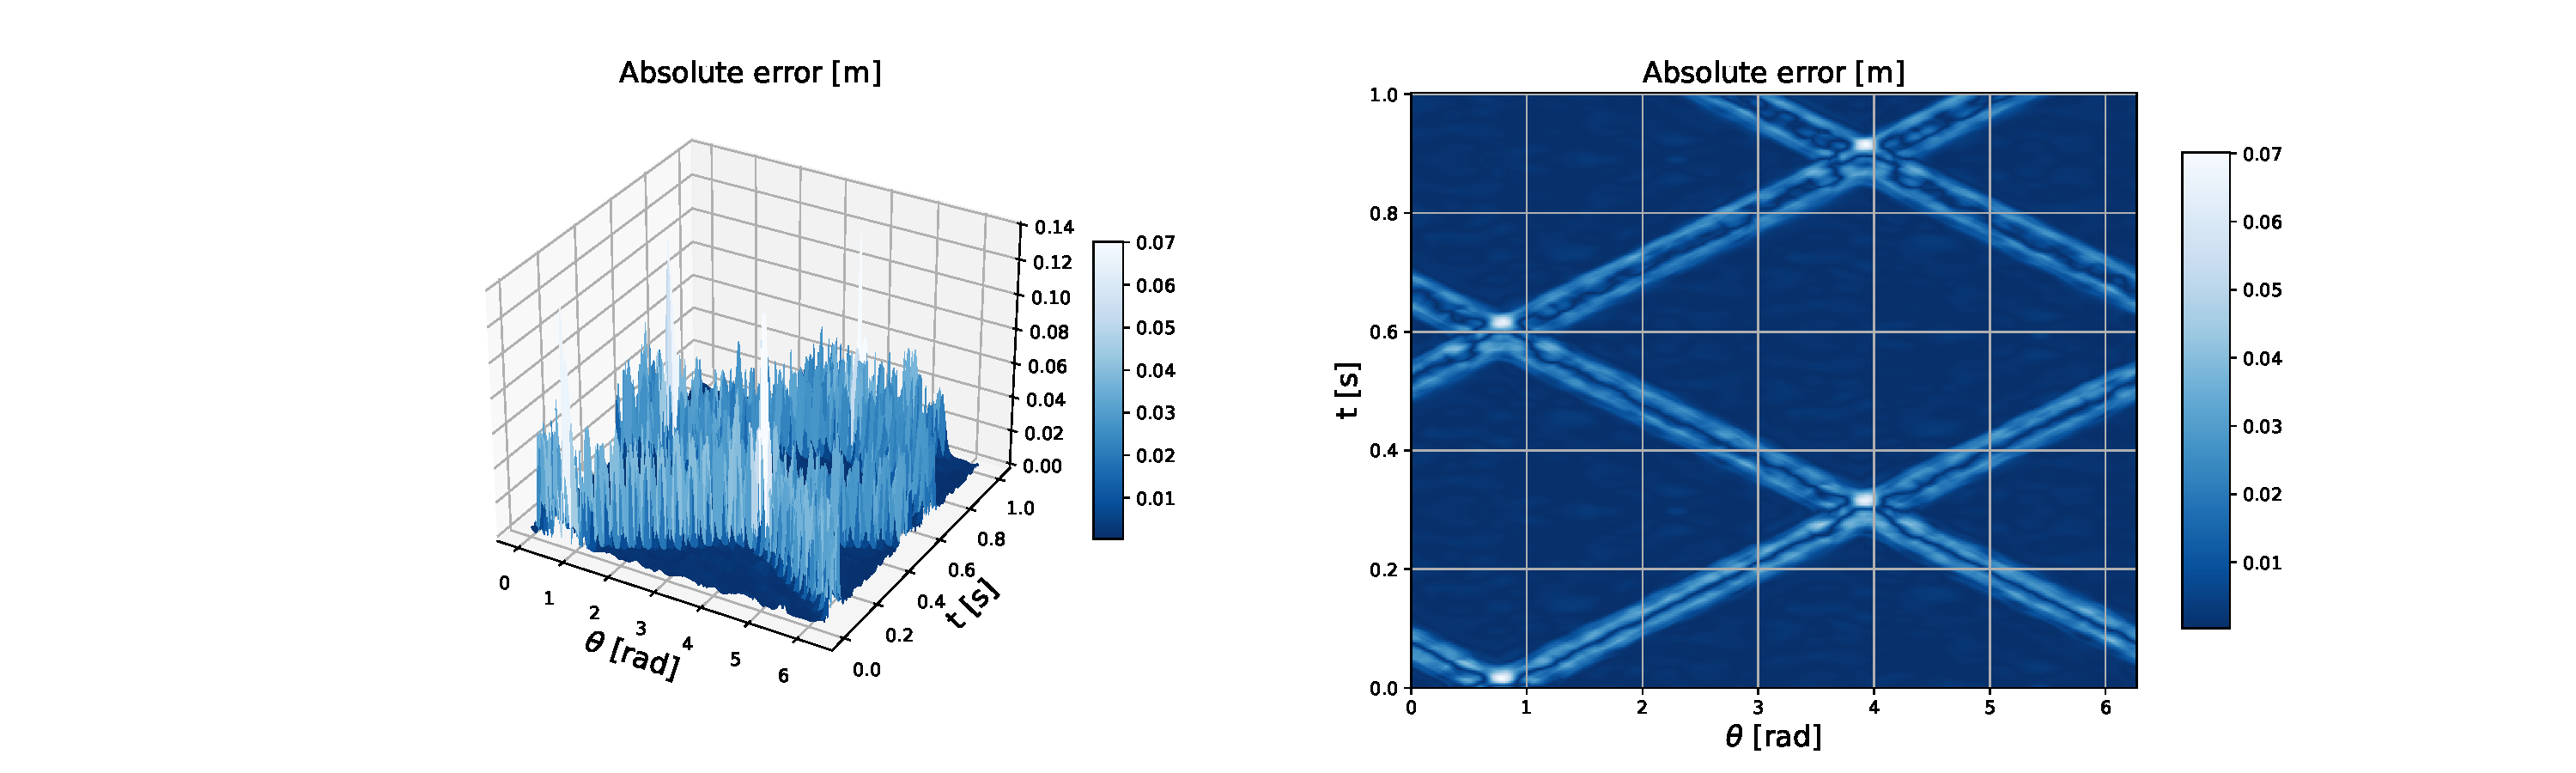
\includegraphics[width=\textwidth]{C:/Users/Matteo/Shallow-Water-Equations/plots/1D_FNO_sphere_error_sigma=2.pdf}
    \caption{Error plots for the predictions of the 1D linearized spherical SWE.}\label{fig:1D_FNO_sphere_error_sigma=2}
\end{figure}
From \autoref{fig:1D_FNO_sphere_error_sigma=2} we see that the model is able to learn the dynamics of the solution.
We also see that the absolute error is biggest at the edges of the solution, which is expected, as the solution tends to be discontinuous.

\begin{figure}[H]
    \centering
    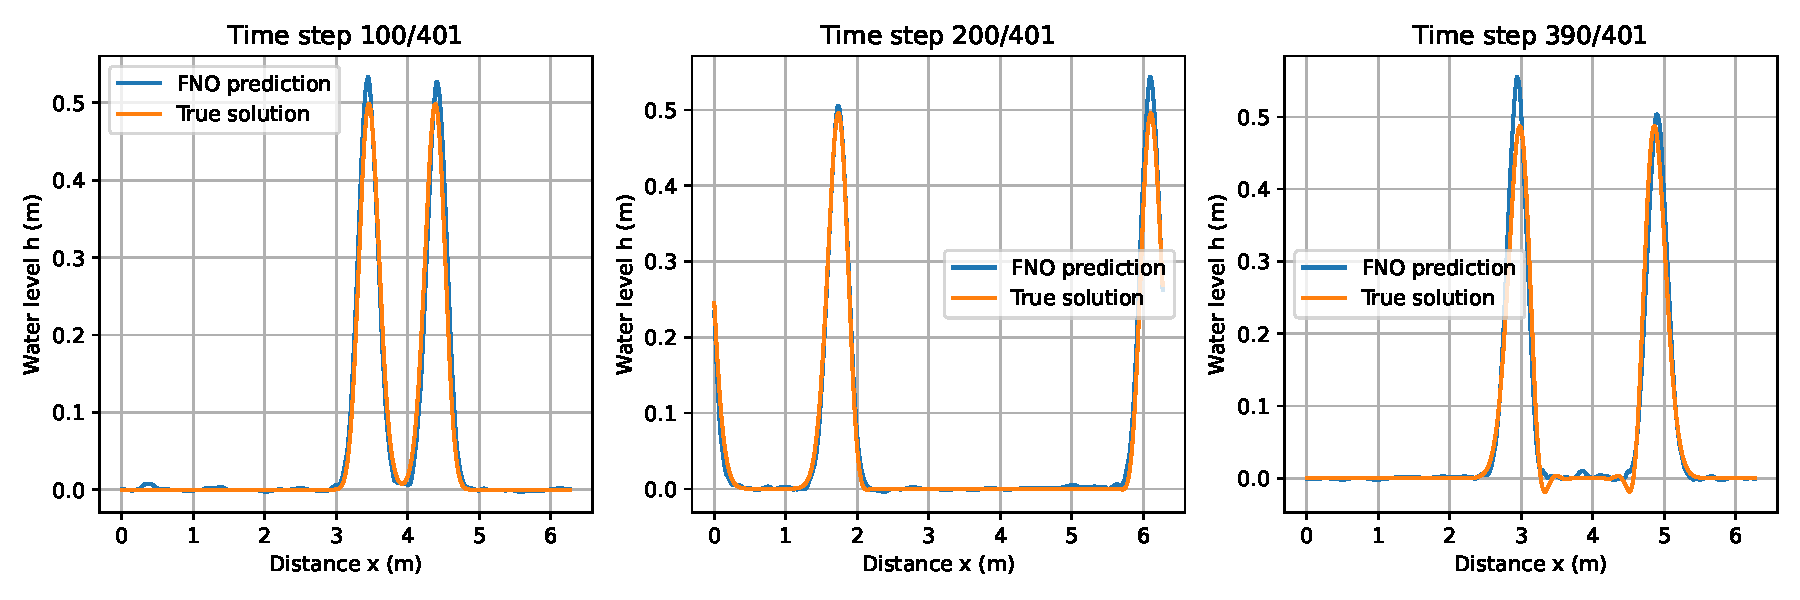
\includegraphics[width=0.9\textwidth]{C:/Users/Matteo/Shallow-Water-Equations/plots/1D_FNO_sphere_pred_timesteps_sigma=2.pdf}
    \caption{Predictions for the spherical shallow water equations in 1D.}\label{fig:1D_FNO_sphere_pred_timesteps_sigma=2}
\end{figure}
From \autoref{fig:1D_FNO_sphere_pred_timesteps_sigma=2} we see that the FNO predictions are smooth and rather accurate, but have some small errors in the top of the waves.

\subsubsection*{Comparison}
To get an overview of the performance of the different models, we consider the MSE for the predictions for the 1D SWE spherical case.
\begin{table}[H]
    \centering
    \small % Reduce font size
    \begin{tabular}{c|ccc|ccc|ccc}
        \hline
        Model & \multicolumn{3}{c|}{$\sigma = \pi/8$} & \multicolumn{3}{c|}{$\sigma = \pi/16$} & \multicolumn{3}{c}{$\sigma = \pi/32$} \\
        \cline{2-10}
        & MSE & MAE & Time (s) & MSE & MAE & Time (s) & MSE & MAE & Time (s) \\
        \hline
        CNN & 
        \input{C:/Users/Matteo/Shallow-Water-Equations/saved_results/1D_CNN_sphere_sigma=1_MSE_test.txt} &
        \input{C:/Users/Matteo/Shallow-Water-Equations/saved_results/1D_CNN_sphere_sigma=1_MAE_test.txt} &
        \input{C:/Users/Matteo/Shallow-Water-Equations/saved_results/1D_CNN_sphere_sigma=1_time.txt} &
        \input{C:/Users/Matteo/Shallow-Water-Equations/saved_results/1D_CNN_sphere_sigma=2_MSE_test.txt} &
        \input{C:/Users/Matteo/Shallow-Water-Equations/saved_results/1D_CNN_sphere_sigma=2_MAE_test.txt} &
        \input{C:/Users/Matteo/Shallow-Water-Equations/saved_results/1D_CNN_sphere_sigma=2_time.txt} &
        \input{C:/Users/Matteo/Shallow-Water-Equations/saved_results/1D_CNN_sphere_sigma=3_MSE_test.txt} &
        \input{C:/Users/Matteo/Shallow-Water-Equations/saved_results/1D_CNN_sphere_sigma=3_MAE_test.txt} &
        \input{C:/Users/Matteo/Shallow-Water-Equations/saved_results/1D_CNN_sphere_sigma=3_time.txt}
        \\ 
        \hline
        FNO & 
        \input{C:/Users/Matteo/Shallow-Water-Equations/saved_results/1D_FNO_sphere_sigma=1_MSE_test.txt} &
        \input{C:/Users/Matteo/Shallow-Water-Equations/saved_results/1D_FNO_sphere_sigma=1_MAE_test.txt} &
        \input{C:/Users/Matteo/Shallow-Water-Equations/saved_results/1D_FNO_sphere_sigma=1_time.txt} &
        \input{C:/Users/Matteo/Shallow-Water-Equations/saved_results/1D_FNO_sphere_sigma=2_MSE_test.txt} &
        \input{C:/Users/Matteo/Shallow-Water-Equations/saved_results/1D_FNO_sphere_sigma=2_MAE_test.txt} &
        \input{C:/Users/Matteo/Shallow-Water-Equations/saved_results/1D_FNO_sphere_sigma=2_time.txt} &
        \input{C:/Users/Matteo/Shallow-Water-Equations/saved_results/1D_FNO_sphere_sigma=3_MSE_test.txt} &
        \input{C:/Users/Matteo/Shallow-Water-Equations/saved_results/1D_FNO_sphere_sigma=3_MAE_test.txt} &
        \input{C:/Users/Matteo/Shallow-Water-Equations/saved_results/1D_FNO_sphere_sigma=3_time.txt}
        \\ 
        \hline
    \end{tabular}
    \caption{Test loss in terms of MSE and MAE, and time for training the models for the 1D spherical SWE.}\label{tab:results_spherical_1D_comparison}
\end{table}
From \autoref{tab:results_spherical_1D_comparison} we see that the CNN model is slightly faster and better than the FNO model for $\sigma = \pi/8$ and $\sigma = \pi/16$, but for $\sigma = \pi/32$, the performance of the CNN model is decreasing.
Probably due to the fact that the smaller the $\sigma$, the more discontinuous the solution is, and the FNO model is better at capturing the discontinuities.
We see that the MAE in general is higher than the MSE, and is also increasing for smaller $\sigma$.
Additionally, we observe that the MAE is higher, as it places more weight on small errors compared to the MSE.
And in the CNN case we see a lot of small errors/noise, which is why the MAE is higher than the MSE.









